\documentclass[9pt,a4paper]{beamer}
\usepackage[utf8]{inputenc}
\usepackage[francais]{babel}
\usepackage[T1]{fontenc}
\usepackage{amsmath}
\usepackage{amsfonts}
\usepackage{amssymb}
\usepackage{makeidx}
\usepackage{graphicx}

\usepackage{color}

\usepackage{listings}

\mode<presentation>

\usetheme{CambridgeUS}

\setbeamertemplate{navigation symbols}{}

\author{\textsc{Frémont} Alexandre et \textsc{Le Calvar} Théo}
\title{Problème des N-Dames}

\begin{document}

\lstdefinestyle{customc}{
  belowcaptionskip=1\baselineskip,
  breaklines=true,
  xleftmargin=\parindent,
  language=C,
  showstringspaces=false,
  basicstyle=\footnotesize\ttfamily,
  keywordstyle=\bfseries\color{green!40!black},
  commentstyle=\itshape\color{purple!40!black},
  identifierstyle=\color{blue},
  stringstyle=\color{orange},
}
\lstset{style=customc}

\begin{frame}
\titlepage
\end{frame}

\begin{frame}
	\frametitle{Plan}
	\tableofcontents
\end{frame}

\section{Introduction}
\begin{frame}

	\begin{block}{Introduction}
	Le problème des N-Dames est une extension du problème des 8 dames, son
	but est de placer 8 dames d’un jeu d’échecs sur un échiquier de façon à ce
	qu’aucune ne soit menacée.

	\end{block}

\end{frame}

\section{Structure de données}
\begin{frame}[fragile]
	\frametitle{Structure de données}
	\begin{block}{Une structure adaptée}
		\begin{itemize}
			\item Code
				\begin{lstlisting}
					typedef struct chessboard {
						size_t          size;
						u32*            queens;
					} cb_t;
				\end{lstlisting}
			\item 	De plus, chaque algorithme apporte ses structures spécialisées.
		\end{itemize}
	\end{block}
\end{frame}

\section{Algorithme CSP}
\begin{frame}
	\frametitle{Algorithmes CSP}

	\begin{block}{Backtracking}
		On construit l'échiquier par étape, lorsque une iteration viole une contrainte on retourne en arrière et on change l'itération.
	\end{block}



	\begin{block}{Forward checking}
		On place nos dames sur l'échiquier et à chaque dame placé on diminue l'espace ou l'on poura placer nos futurs dames. \\
		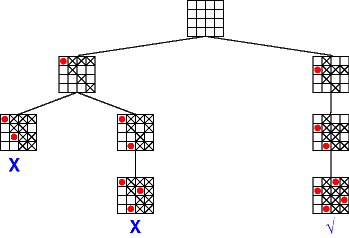
\includegraphics[width=0.4\textwidth]{images/forw.png}
	\end{block}

\end{frame}


\section{Algorithme de recherche locale}
\begin{frame}
	\frametitle{Algorithme de recherche locale}

	\begin{block}{1er algorithme de recherche local}
		\begin{itemize}
			\item{initialisation}
			\item{transposition entre les dames en conflits seulement}
			\item{descente stricte}
		\end{itemize}
	\end{block}

	\begin{block}{2nd algorithme de recherche local}
		\begin{itemize}
		      \item{initialisation avec un nombre réduit de conflits}
		      \item{transposition entre les dames en conflits seulement}
		      \item{descente stricte}
	      \end{itemize}
	\end{block}



\end{frame}

\section{Resultats et performance}
\begin{frame}
	\frametitle{Backtracking}

	\hspace{0.8cm} 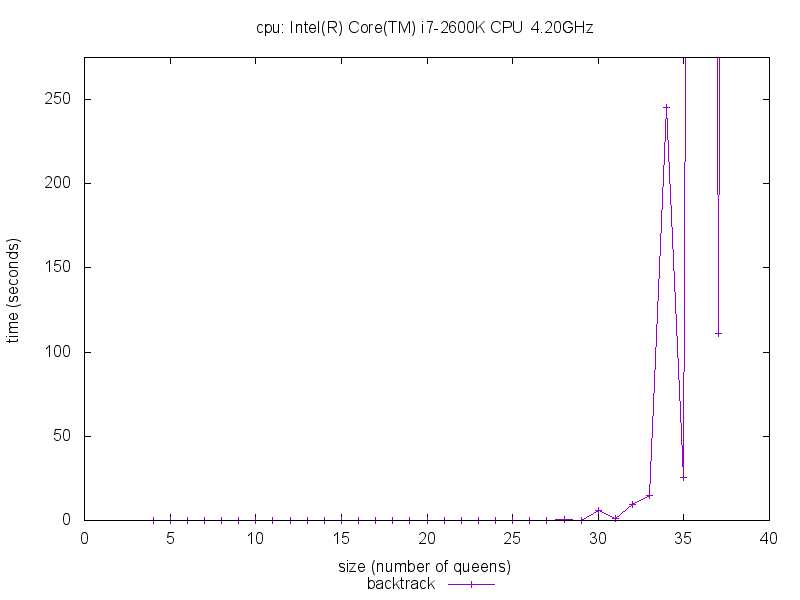
\includegraphics[height=0.9\textheight]{images/plot_bt_i7.png}

\end{frame}

\begin{frame}
	\frametitle{Forward Checking}
	\hspace{0.8cm} 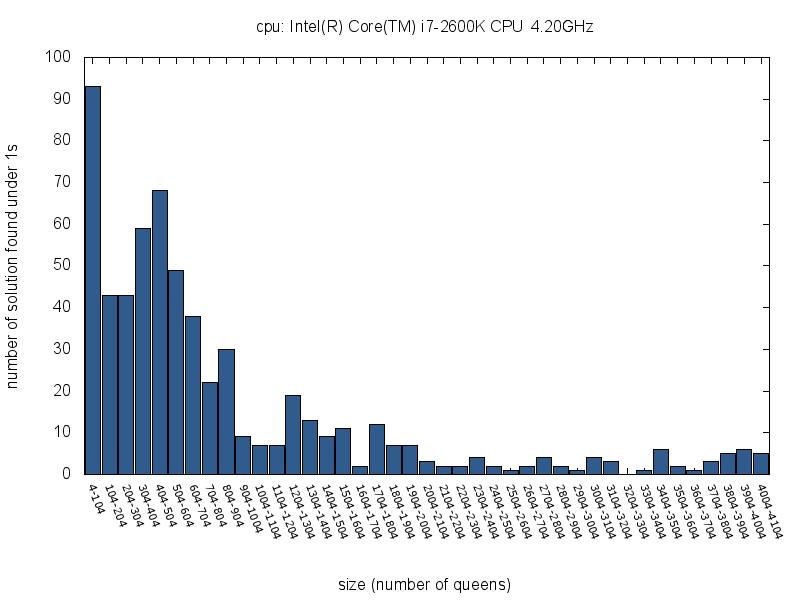
\includegraphics[height=0.9\textheight]{images/plot_fw_i7.png}

\end{frame}

\begin{frame}
	\frametitle{Comparaison backtracking-forward checking}
	\hspace{0.8cm} 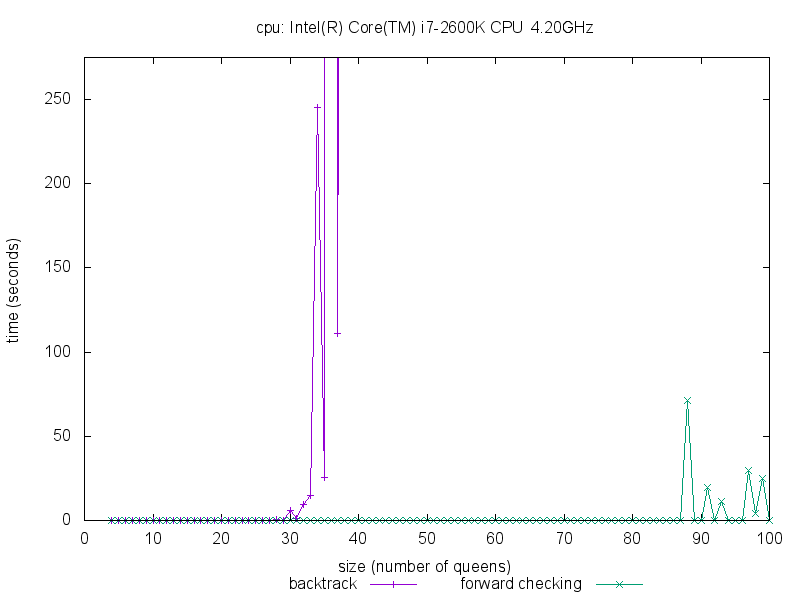
\includegraphics[height=0.9\textheight]{images/plot_bt_fw_i7.png}
\end{frame}

\begin{frame}
	\frametitle{Local search 1}

	\hspace{0.8cm} 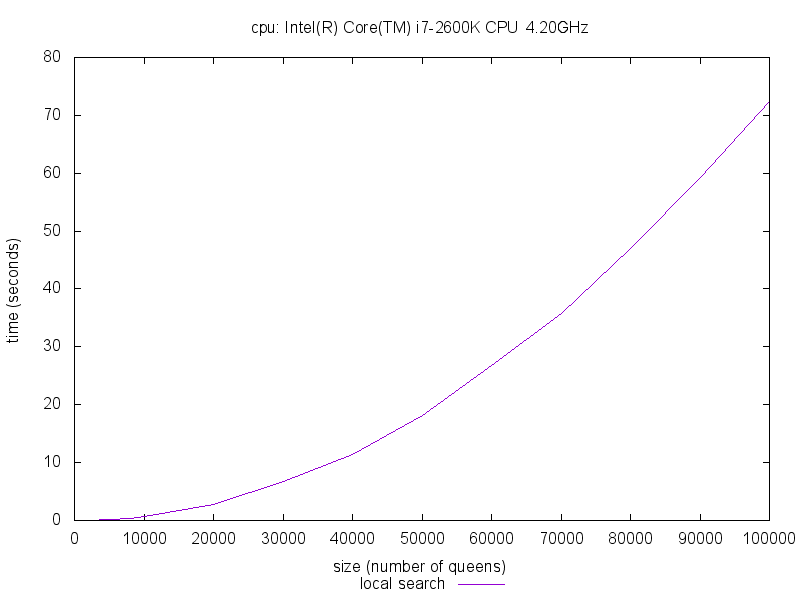
\includegraphics[height=0.9\textheight]{images/plot_ls_i7.png}
\end{frame}

\begin{frame}
	\frametitle{Local Search 2}

	\hspace{0.8cm} 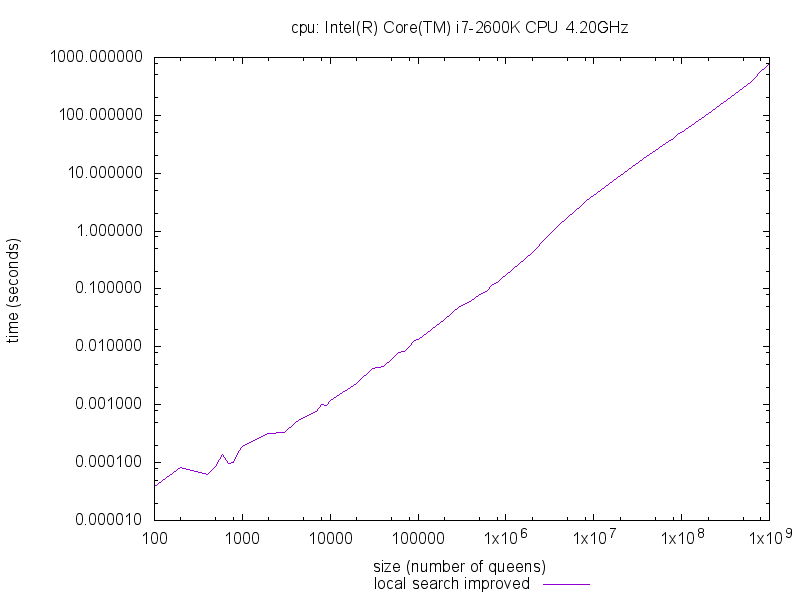
\includegraphics[height=0.9\textheight]{images/plot_lst_i7.png}
\end{frame}

\begin{frame}
	\frametitle{Comparaison local search 1 \& 2}

	\hspace{0.8cm} 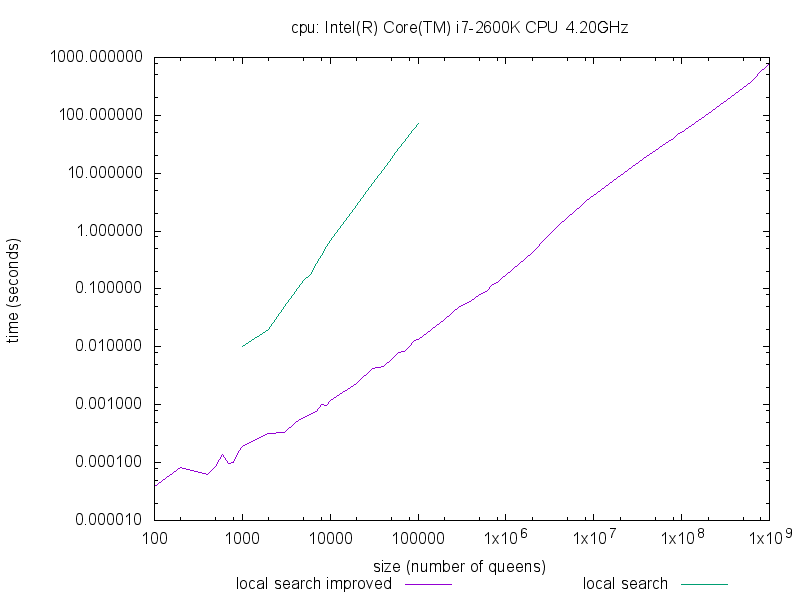
\includegraphics[height=0.9\textheight]{images/plot_lst_ls_i7.png}
\end{frame}

\section{Conclusion}
\begin{frame}
	\frametitle{Conclusion}

	\begin{block}{Avantages et inconvenients}
	      \begin{itemize}
			\item{Backtracking et Forward Checking, un résultat certain mais sans certitude d'un temps d'exécution raisonnable.\footnote{\textit{Deep Thought} et ses 7.5 millions d'années.}}
			\item{Methode de recherche local, résultat statistiquement incertain mais dans la pratique, temps raisonnable.}
	      \end{itemize}

	\end{block}
\end{frame}

\begin{frame}
	\frametitle{Bonus}

	Visualisation de solutions.
\end{frame}


\end{document}
